% Matematik 2b – Prövningsprov
% Skapat med samma struktur som Matematik 1b-provet

\documentclass[a4paper,11pt]{article}
\usepackage[utf8]{inputenc}
\usepackage[T1]{fontenc}
\usepackage[swedish]{babel}
\usepackage{amsmath,amssymb,amsfonts}
\usepackage{tikz}
\usetikzlibrary{calc}
\usetikzlibrary{intersections, through}
\usepackage{pgfplots}
\pgfplotsset{compat=1.17}
\usepackage{enumitem}
\usepackage{geometry}
\geometry{margin=2.5cm}

\title{Prövningsprov Matematik 2b}
\author{Viktor Arohlén}
\date{\today}

\begin{document}

\maketitle

% --- Information och regler ---
\begin{center}
\fbox{\parbox{0.93\textwidth}{
\textbf{Viktiga regler för provet:}
\begin{itemize}
    \item \textbf{Del A (utan digitala verktyg):} Här får du endast använda formelblad och linjal. Miniräknare, GeoGebra eller andra digitala hjälpmedel är inte tillåtna.
    \item \textbf{Del B (med digitala verktyg):} Här får du använda miniräknare, GeoGebra och andra digitala verktyg.
    \item Skriv tydliga lösningar och motivera alla steg.
    \item Mobiltelefoner och kommunikation är ej tillåtet.
    \item Toalettbesök endast mellan provdelarna.
    \item Misstänkt fusk leder till att provet ej kan bedömas.
\end{itemize}
}}
\end{center}

\begin{center}
\fbox{\parbox{0.93\textwidth}{
Jag skriver under på att jag tagit del av reglerna ovan och följer dem:

\vspace{2mm}
\textbf{Namn:}\hrulefill\hspace{1cm}\textbf{Klass:}\hrulefill
}}
\end{center}



% --- Del B: Utan digitala hjälpmedel ---
\newpage
\section*{Del A: Utan digitala hjälpmedel}
\begin{enumerate}[label=\arabic*.]
    \item Förenkla uttrycket: $(2x - 3)(x + 5)$
    \item Utveckla och förenkla: $(y + 4)^2 - (y - 4)^2$
    % Tolkning av andragradsgraf
    \item Nedan visas grafen till andragradsfunktionen $y = f(x)$. 
    \begin{enumerate}[label=\alph*)]
      \item Ange symmetrilinjens ekvation
      \item Ange funktionens nollställen
    \end{enumerate}
    \begin{center}
    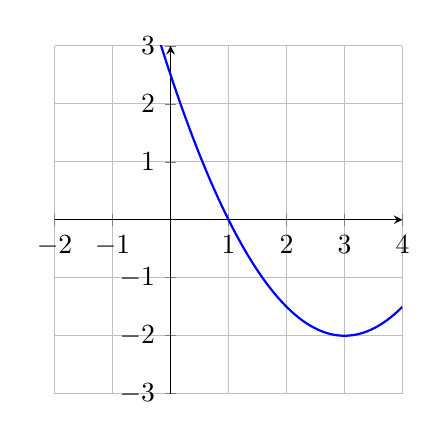
\begin{tikzpicture}
      \begin{axis}[
        axis lines=middle,
        axis line style/.append style={-},
        grid=both,
        xmin=-2, xmax=4,
        ymin=-3, ymax=3,
        samples=200,
        width=6cm,
        height=6cm,
        domain=-1:4,
        xtick distance=1,
        ytick distance=1,
        clip=true
      ]
        \addplot[blue, thick] {0.5 * (x-1) * (x-5)};
      \end{axis}
    \end{tikzpicture}
    \end{center}
    \item Lös ekvationerna och svara exakt:
    \begin{enumerate}[label=\alph*)]
        \item $3^{2x} = 17$
        \item $3x^2 + 6x = 0$
        \item $\lg x = 4$
        \item $2x^2 - 20x + 50 = 0$
    \end{enumerate}
    \item Lös ekvationssystemet:
    \[
    \left\{
    \begin{array}{l}
      2x + y = 11 \\
      x - y = 1
    \end{array}
    \right.
    \]
    % Implikation och ekvivalens
    \item Avgör vilken symbol som ska stå mellan påståendena: implikation ($\Rightarrow$ eller $\Leftarrow$) eller ekvivalens ($\Leftrightarrow$). Skriv rätt symbol på linjen. Om inget samband finns, skriv "ingen".
    
    \begin{center}
    \renewcommand{\arraystretch}{1.6}
    \begin{tabular}{l c l}
      a) $x > 2$ & \rule{1.5cm}{0.15mm} & $x^2 > 4$ \\
      b) ''P är en rektangel'' & \rule{1.5cm}{0.15mm} & ''P är en kvadrat'' \\
      c) $x = 5$ & \rule{1.5cm}{0.15mm} & $10x = 50$ \\
    \end{tabular}
    \end{center}
    \item Ett rektangulärt fält har en längd som är 2 meter längre än dess bredd. Om arean av fältet är 15 m², bestäm längden och bredden på fältet.

    \newpage
    \item Två kordor skär varandra i en cirkel enligt figuren nedan. Beräkna $x$.
    \begin{center}
    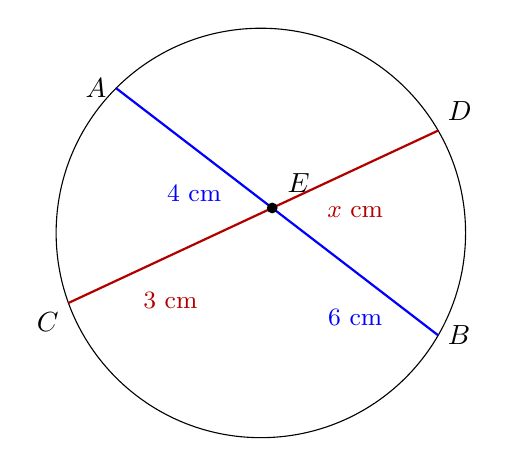
\begin{tikzpicture}[scale=1.3]
      \draw (0,0) circle (2cm);
      % Punkter på cirkeln
      \coordinate (A) at ({2*cos(135)},{2*sin(135)});
      \coordinate (B) at ({2*cos(330)},{2*sin(330)});
      \coordinate (C) at ({2*cos(200)},{2*sin(200)});
      \coordinate (D) at ({2*cos(30)},{2*sin(30)});
      % Skärningspunkt mellan AB och CD
      \path[name path=AB] (A) -- (B);
      \path[name path=CD] (C) -- (D);
      \path [name intersections={of=AB and CD, by=E}];
      % Rita kordor
      \draw[thick,blue] (A) -- (intersection-1) -- (B);
      \draw[thick,red!70!black] (C) -- (intersection-1) -- (D);
      \fill (intersection-1) circle (1.5pt);
      % Noder
      \node[left] at (A) {$A$};
      \node[right] at (B) {$B$};
      \node[below left] at (C) {$C$};
      \node[above right] at (D) {$D$};
      \node[above right=2pt] at (intersection-1) {$E$};
      % Mått
      % Måttetiketter placerade under linjerna
      \node[blue,below=10pt] at ($ (A)!0.5!(intersection-1) $) {\small 4 cm};
      \node[blue,below=10pt] at ($ (intersection-1)!0.5!(B) $) {\small 6 cm};
      \node[red!70!black,below=10pt] at ($ (C)!0.5!(intersection-1) $) {\small 3 cm};
      \node[red!70!black,below=10pt] at ($ (intersection-1)!0.5!(D) $) {\small $x$ cm};
    \end{tikzpicture}
    \end{center}



    % Uppgift 10 – Problemlösning med ekvationssystem
    \item Anna köper 3 äpplen och 2 päron för 22 kr. Erik köper 2 äpplen och 4 päron för 24 kr. Vad kostar ett äpple och vad kostar ett päron?


% --- Del B: Uppgifter med digitala verktyg ---
\newpage
\section*{Del B – Uppgifter med digitala verktyg}

% 1. Problemlösning med andragradsfunktion (exempel: bro)
\item En bro har formen av en andragradsfunktion: $y = -0,5x^2 + 4x$. Med hjälp av GeoGebra, bestäm brospannets bredd (avståndet mellan de två punkter där bron möter marken, dvs. där $y=0$) och den maximala höjden på bron.

% 2. Statisk värdeuppgift (GeoGebra)
\item I en tabell har du följande värden för $x$ och $y$:

\begin{tabular}{|c|c|c|c|c|}
\hline
$x$ & 1 & 2 & 3 & 4 \\
\hline
$y$ & 5 & 7 & 9 & 11 \\
\hline
\end{tabular}

Använd GeoGebra för att undersöka sambandet mellan $x$ och $y$. Vilken typ av funktion passar bäst? Vad blir $y$ när $x=6$?

% 3. Normalfördelningsuppgift
\item Längden på morötter i en odling är normalfördelad med medelvärde $18$ cm och standardavvikelse $2$ cm. Använd ett digitalt verktyg för att uppskatta hur stor andel av morötterna som är längre än $20$ cm.

% 4. Exponentialfunktion (bävrar)
\item En bäverpopulation minskar med $8\%$ per år. Från början finns det $150$ bävrar. Skriv en exponentialfunktion som beskriver antalet bävrar $n$ år efter start, och beräkna hur många bävrar det finns efter $5$ år.

\item Lös ekvationerna, svara med två decimaler
\begin{enumerate}[label=\alph*)]
    \item $7^{\frac{x}{5}} = 1,3$
    \item $2^x = 7$
    \item $x^2 - 5x + 2 = 0$
    \item $3x^2 = 8x - 1$
\end{enumerate}

\end{enumerate}

\end{document}
